\subsection{Ordnungsrelationen}
\begin{def*}[note = Partialordnung , index = Partialordnung]
	Eine Relation $\enquote{\leq}$ auf $A$ heisst Partialordnung, falls sie
	\begin{itemize}
		\item reflexiv,
		\item antisymmetrisch und
		\item transitiv
	\end{itemize}
	ist.
\end{def*}
\begin{bsp*}
	\begin{itemize}
		\item $\mathbb{N}, \mathbb{Z}, \mathbb{R} \text{ mit } \leq, \geq$
		\item $| \text{ auf } \mathbb{N}$ \\
			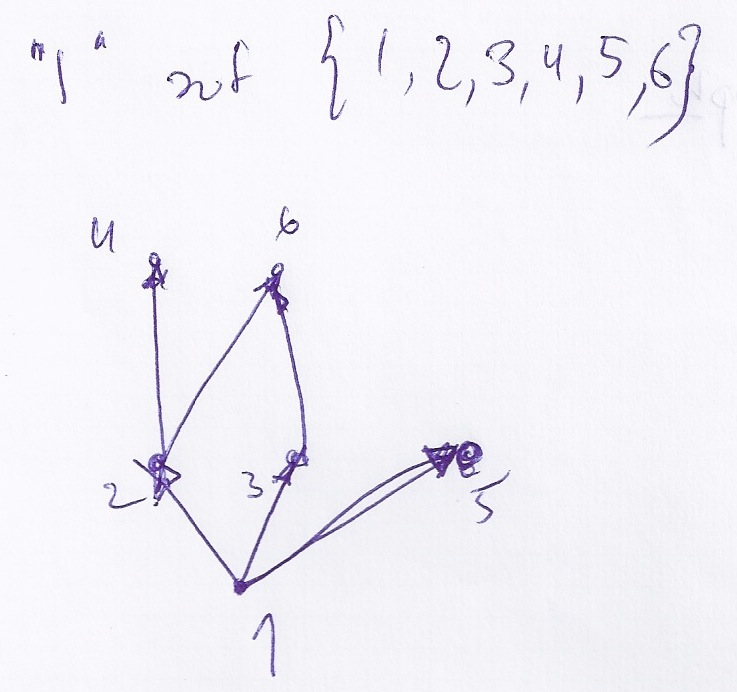
\includegraphics{Bild19} \\
			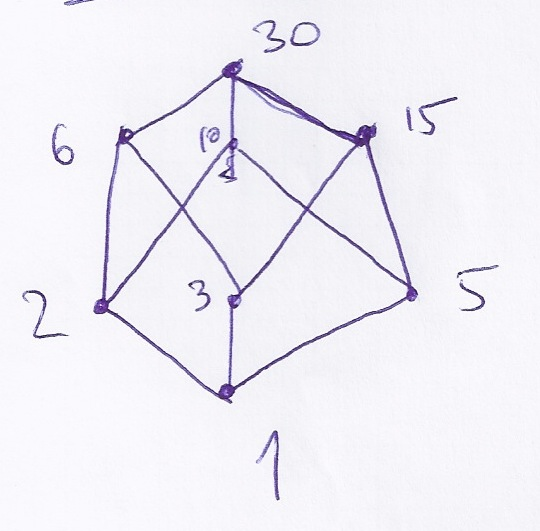
\includegraphics{Bild20}
		\item $\subseteq \text{ auf } \mathbb{P}( B ) \text{ für eine Menge } B$ \\
			
\includegraphics{Bild21}
	\end{itemize}
\end{bsp*}
\todo{Too long}
\begin{bem}
	Nicht jedes Paar von Objekten muss vergleichbar sein.\\
	Falls es so ist, spricht man von einer \textbf{linearen}\index{Ordnung!lineare} oder \textbf{totalen}\index{Ordnung!totale} Ordnung, \textbf{Kette}\index{Kette}.
\end{bem}
\begin{def*}[note = vergleichbar , index = vergleichbar]
	$x$ und $y$ \textbf{vergleichbar}, falls $x \leq y \vee y \leq x$
\end{def*}

\subsubsection{Wichtige Begriffe}
\begin{def*}[note = maximales Element , index = Element!maximales]
	$x$ \textbf{maximales Element} falls \\
	\[ \not\exists y \neq x : y \geq x \qquad (\not\exists y : y > x) \qquad y > x :\iff y \geq x \wedge y \neq x \]
	analog: \textbf{minimales Element}\index{Element!minimales}
\end{def*}
\begin{def*}[note = grösstes Element , index = Element!grösstes]
	$x$ \textbf{grösstes Element} falls \\
	\[ \forall y \leq x \]
	analog: \textbf{kleinstes Element}\index{Element!kleinstes}
\end{def*}
\begin{def*}[note = wohlgeordnet , index = wohlgeordnet]
	$(A, \leq)$ heisst \textbf{wohlgeordnet (WO)} falls jede nichtleere Teilmenge ein kleinstes Element hat. \\
	\begin{bsp*}{wohlgeordnete Ordnungsrelation}
		\[ (\mathbb{N}, \leq ) \]
	\end{bsp*}
	\begin{bsp*}{keine WO}
		\begin{itemize}
			\item $(\mathbb{Z}, \leq )$
			\item $([0,1], \leq)$
		\end{itemize}
	\end{bsp*}
\end{def*}

\subsubsection{Hasse-Diagramme}
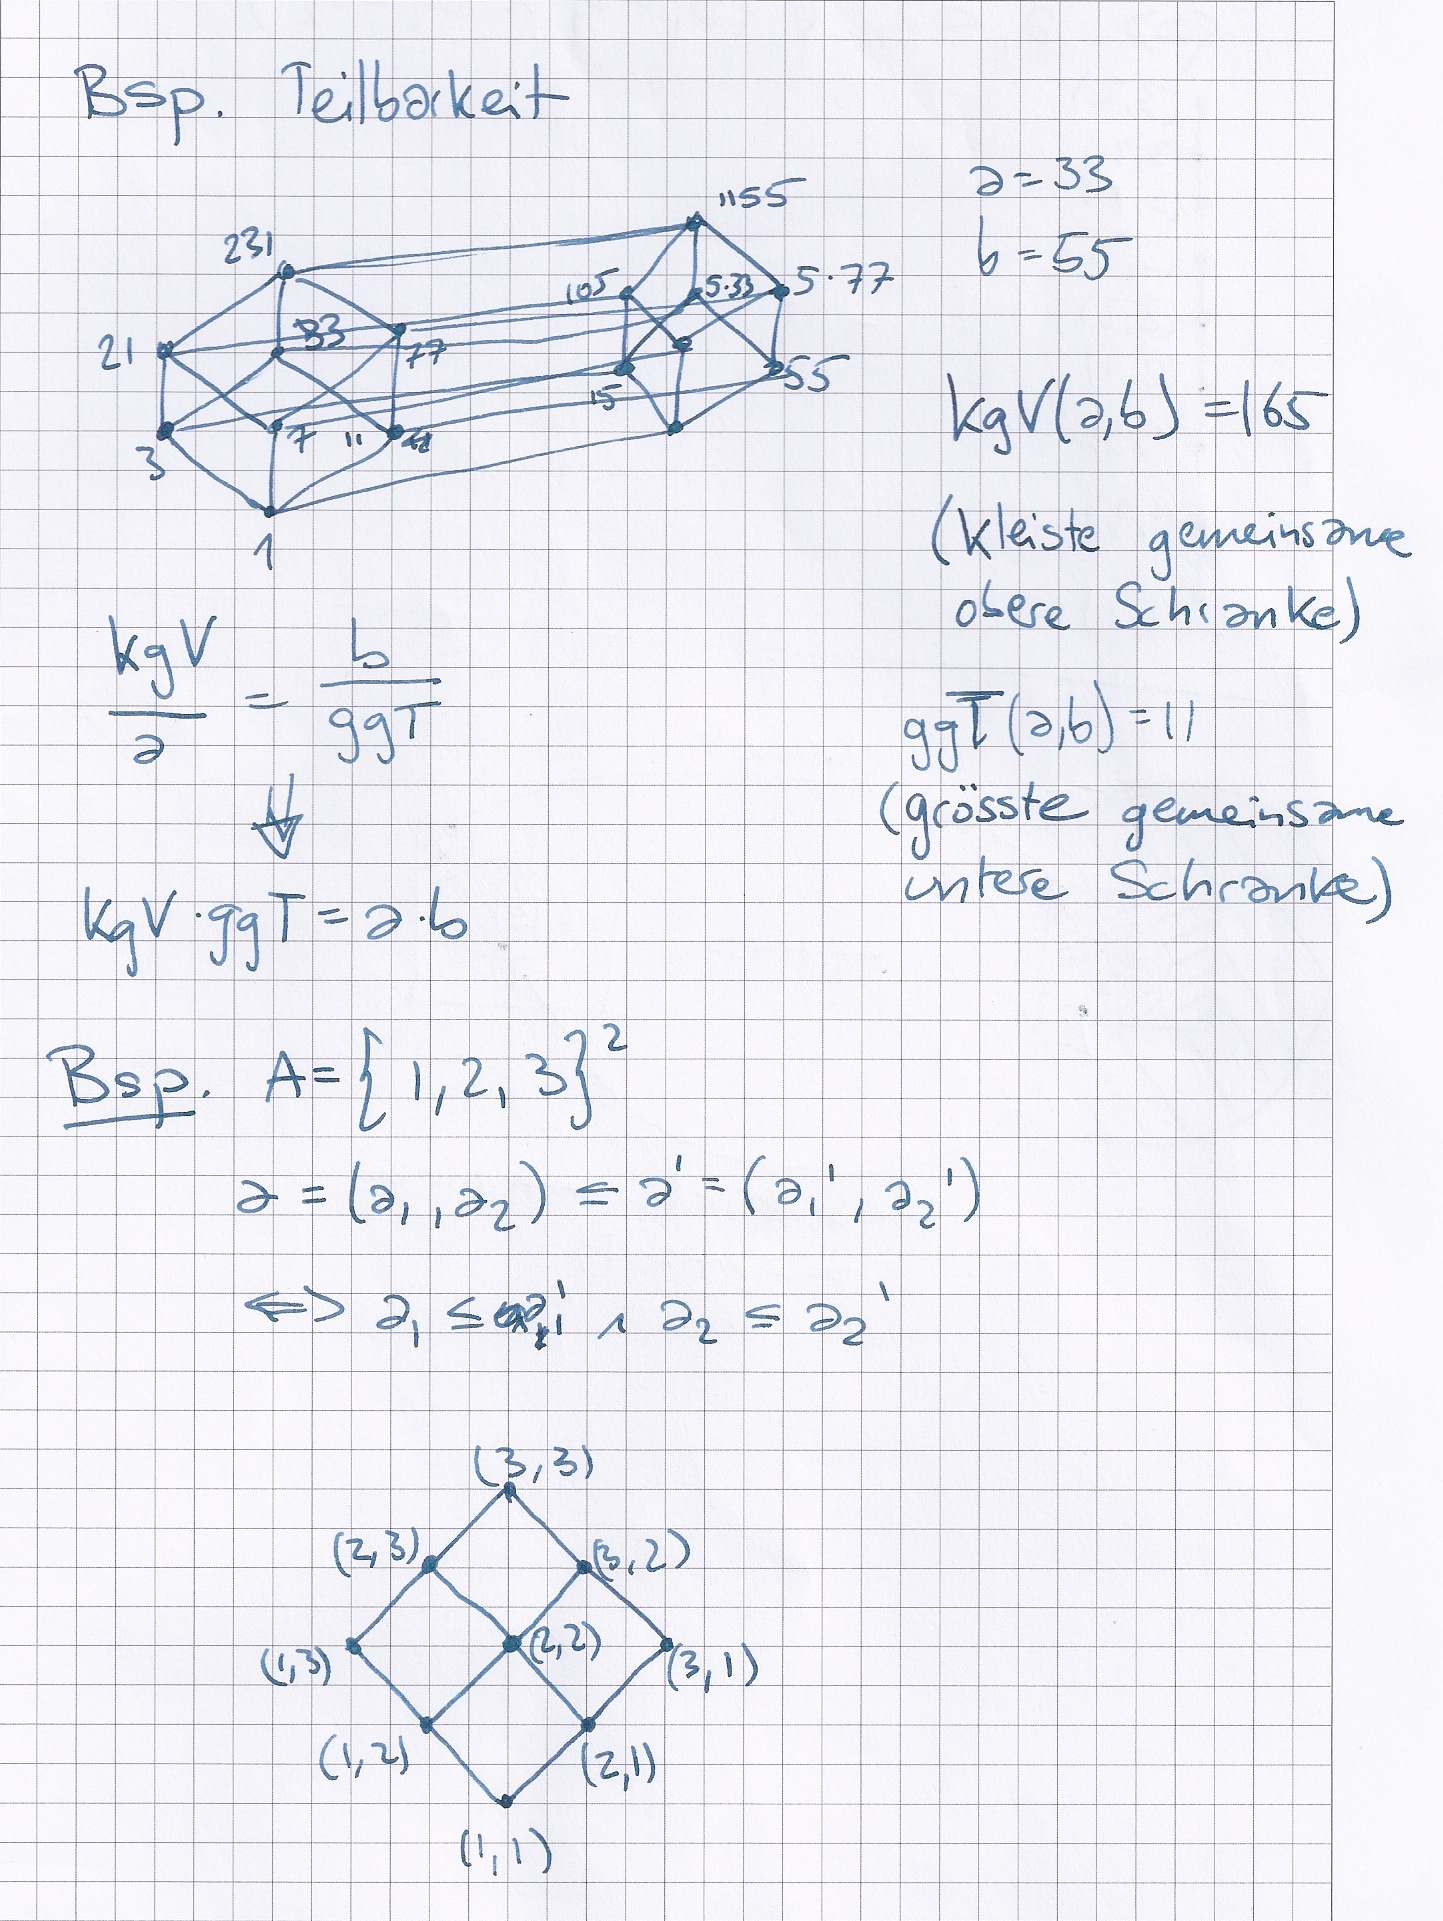
\includegraphics[width=\textwidth]{Bild22}
\begin{itemize}
	\item Es werden nur direkte Nachbarn verbunden $( x \leq y \text{ direkte Nachbarn }: x \neq y \wedge \not\exists z : x < z < y )$
	\item Orientierung durch Position ( unten $\leq$ oben )
\end{itemize}